\section{Squark Production at One-Loop}


\subsection{The LSZ Theorem}\label{sec:LSZ}
The LSZ theorem\cite{Lehmann:1954rq} or LSZ reduction formula prescribes how to obtain the S-matrix element, i.e. a physical observable, from the time ordered correlation function of the respective field operators. The time ordered correlation function of fields in an interacting theory can be calculated perturbatively with the aid of the Gell-Mann and Low theorem and the Wick theorem. \\
Considering a physical process with kinematics $\vec{k}_1 \hdots \vec{k}_n \to \vec{p}_1 \hdots \vec{p}_m$ and taking for the sake of simplicity only one scalar field $\phi$ the Fourier transform of the time ordered product of a correlation function is related to the corresponding S-matrix element like\footnote{In this subsection the $\sim$ indicates that the poles on either side are the same provided that all momenta are close to their mass shell, i.e. $p_i^0 \to E_{\vec{p}_i}$ and $k_j^0 \to E_{\vec{k}_j}$.}
\begin{align}
\prod_{i=1}^n \int \mathrm{d}x_i\ \mathrm{e}^{ip_i x_i} \prod_{j=1}^m \int \mathrm{d}y_j\ \mathrm{e}^{ik_j y_j} \left\langle \Omega | \mathcal{T} \left[ \phi(x_1) \hdots \phi(x_n) \phi(y_1) \hdots \phi(y_m) \right] | \Omega\right\rangle \nonumber\\
\sim \prod_{i=1}^n \frac{i\sqrt{Z}}{p_i^2 - m^2 + i\epsilon} \prod_{j=1}^m \frac{i\sqrt{Z}}{k_j^2 - m^2 + i\epsilon} \left\langle \left.\left.\vec{p}_1 \hdots \vec{p}_n \right| S \right| \vec{k}_1 \hdots \vec{k}_m \right\rangle .\label{eq:LSZ}
\end{align}
Here $\mathcal{T}$ denotes the time ordering operator, $\left.| \Omega \right\rangle$ is the ground state of the interacting theory and $\sqrt{Z}$ is the residue of the single particle pole in the two-point function 
\begin{align}
\int \mathrm{d}x\ \mathrm{e}^{ip x} \left\langle \Omega | \mathcal{T} \left[ \phi(x) \phi(0) \right] | \Omega\right\rangle &= \frac{i}{p^2-m_0^2} + \frac{i}{p^2-m_0^2} \left(\frac{i\Sigma(p^2)}{p^2-m_0^2}\right) + \frac{i}{p^2-m_0^2} \left(\frac{\Sigma(p^2)}{p^2-m_0^2}\right)^2 + \hdots\nonumber\\
&= \frac{i}{p^2 - m_0^2 - \Sigma(p^2)}.\label{eq:propagator}
\end{align}
\begin{figure}[!htbp]
\begin{center}
\begin{tikzpicture}[line width=2.0 pt, scale=1.3]
	\draw[fermionnoarrow](180:1)--(180:0.5);	
	\draw (0,0) circle (.5cm);
		\begin{scope}
	    	\clip (0,0) circle (.5cm);
	    	\foreach \x in {-1.0,-0.9,...,1.0}
        \draw[line width=1 pt] (\x,-.5) -- (\x+.6,.5);
	  	\end{scope}
	\draw[fermionnoarrow](0:0.5)--(0:1);
	\node at (1.3,0) {=};
	\draw[fermionnoarrow](0:1.6)--(0:2.6);
	\node at (2.9,0) {+};
    \draw[fermionnoarrow](0:3.2)--(0:3.7);	
	\draw (4.2,0) circle (.5cm);
	\node at (4.2,0) {1PI};
	\draw[fermionnoarrow](0:4.7)--(0:5.2);
	\node at (5.5,0) {+};	
	\draw[fermionnoarrow](0:5.8)--(0:6.3);	
	\draw (6.8,0) circle (.5cm);
	\node at (6.8,0) {1PI};
	\draw[fermionnoarrow](0:7.3)--(0:7.8);
	\draw (8.3,0) circle (.5cm);
	\node at (8.3,0) {1PI};
	\draw[fermionnoarrow](0:8.8)--(0:9.3);
	\node at (9.8,0) {+ $\hdots$};
\end{tikzpicture}
\caption{Diagrammatic figure of the two-point function of a scalar field: The propagator in an interaction theory can be calculated in a perturbation series in the coupling constant.}\label{fig:fullpropagator}
\end{center}
\end{figure}
The parameter $m_0$ is the tree-level mass and the quantity $-i \Sigma(p^2)$ denotes the sum of all one-particle-irreducible contributions to the particle's self-energy. From eq. \eqref{eq:propagator} one can read off the physical mass $m^2$ of the particle which is associated with the field $\phi$. It is determined as the value of $p^2$ where the propagator has a pole, i.e. 
\begin{align}
\left[ p^2 - m_0^2 - \Sigma(p^2)\right]_{p^2 = m^2} = 0
\end{align}
Close to the pole the denominator of eq. \eqref{eq:propagator} can by expanded like
\begin{align}
p^2 - m_0^2 - \Sigma(p^2) = (p^2 - m^2)\left( 1 - \frac{\partial \Sigma(p^2)}{\partial p^2} \right)_{p^2 = m^2} + \mathcal{O}((p^2 - m^2)^2).
\end{align}
The residue of the propagator can therefore be written as 
\begin{align}
Z = \left( 1 - \frac{\partial \Sigma(p^2)}{\partial p^2} \right)_{p^2 = m^2}^{-1}.
\end{align}
Now considers the full $(n+m)$-point function in scalar theory. One can decompose it into an amputated $(n+m)$-point function and ``full'' propagators like written in eq. \eqref{eq:propagator} and depicted in fig. \ref{fig:fullpropagator}.
\begin{figure}[!htbp]
\begin{center}
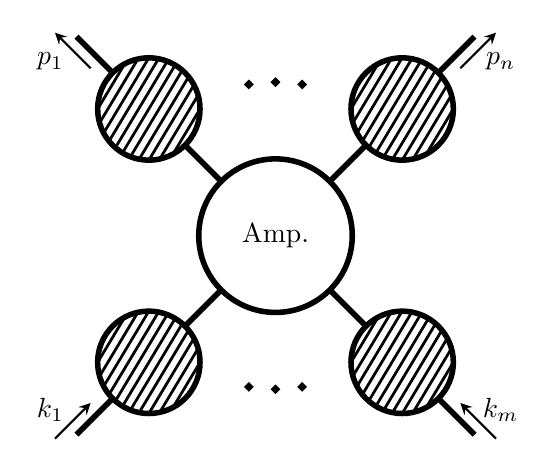
\begin{tikzpicture}[line width=2.0 pt, scale=1.3, arrow/.style={thick,->,shorten >=2pt,shorten <=2pt,>=stealth}]
	\draw (0,0) circle (.75);
	\node at (0,0) {Amp.};
	\draw (45:0.75)--(45:1.25);
	\draw (45:1.75) circle (.5);
		\begin{scope}[shift={(45:1.75)}]
	    	\clip (0,0) circle (.5cm);
	    	\foreach \x in {-1.0,-0.9,...,1.0}
        \draw[line width=1 pt] (\x,-.5) -- (\x+.6,.5);
	  	\end{scope}
	\draw (45:2.25)--(45:2.75);
	\draw[arrow] (1.768,1.597)--(2.192,2.021);
	\node at (2.2,1.7){$p_n$};

	\draw (135:0.75)--(135:1.25);
	\draw (135:1.75) circle (.5);
		\begin{scope}[shift={(135:1.75)}]
	    	\clip (0,0) circle (.5cm);
	    	\foreach \x in {-1.0,-0.9,...,1.0}
        \draw[line width=1 pt] (\x,-.5) -- (\x+.6,.5);
	  	\end{scope}
	\draw (135:2.25)--(135:2.75);
	\draw[arrow] (-1.768,1.597)--(-2.192,2.021);
	\node at (-2.2,1.7){$p_1$};	
	
	\draw (225:0.75)--(225:1.25);
	\draw (225:1.75) circle (.5);
		\begin{scope}[shift={(225:1.75)}]
	    	\clip (0,0) circle (.5cm);
	    	\foreach \x in {-1.0,-0.9,...,1.0}
        \draw[line width=1 pt] (\x,-.5) -- (\x+.6,.5);
	  	\end{scope}
	\draw (225:2.25)--(225:2.75);
	\draw[arrow] (-2.192,-2.021)--(-1.768,-1.597);
	\node at (-2.2,-1.7){$k_1$};	
	
	\draw (315:0.75)--(315:1.25);
	\draw (315:1.75) circle (.5);
		\begin{scope}[shift={(315:1.75)}]
	    	\clip (0,0) circle (.5cm);
	    	\foreach \x in {-1.0,-0.9,...,1.0}
        \draw[line width=1 pt] (\x,-.5) -- (\x+.6,.5);
	  	\end{scope}
	\draw (315:2.25)--(315:2.75);
	\draw[arrow] (2.192,-2.021)--(1.768,-1.597);
	\node at (2.2,-1.7){$k_m$};
	
	\draw[fill=black] (80:1.5) circle (.01);
	\draw[fill=black] (90:1.5) circle (.01);
	\draw[fill=black] (100:1.5) circle (.01);
	\draw[fill=black] (-80:1.5) circle (.01);
	\draw[fill=black] (-90:1.5) circle (.01);
	\draw[fill=black] (-100:1.5) circle (.01);
\end{tikzpicture}
\caption{Diagrammatic figure of a ``full' $(n+m)$-point function. Apart from the ``full'' propagators there is the ``full'' amputated $(n+m)$-point function}
\end{center}
\end{figure}\\
Inserting the expression
\begin{align}
\frac{i}{p^2 - m_0^2 - \Sigma(p^2)} \sim \frac{i Z}{p^2 - m^2}
\end{align}
for the full propagators one notices the same singularity as in eq. \eqref{eq:LSZ}. If one now compares the coefficients of these poles in eq. \eqref{eq:LSZ} one finds
\begin{figure}[!htbp]
\begin{center}
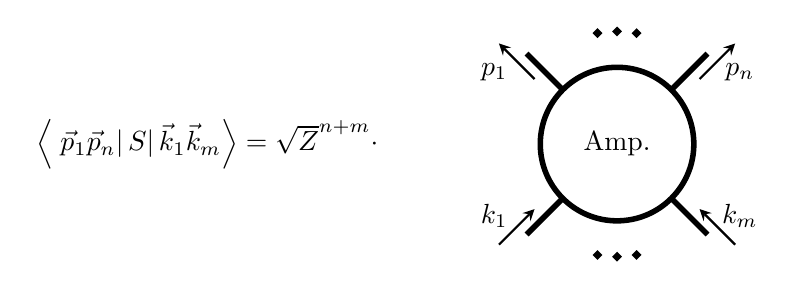
\begin{tikzpicture}[line width=2.0 pt, scale=1.3, arrow/.style={thick,->,shorten >=2pt,shorten <=2pt,>=stealth}]
	\node at (-4,0) {$\left\langle \left.\left.\vec{p}_1 \hdots \vec{p}_n \right| S \right| \vec{k}_1 \hdots \vec{k}_m \right\rangle =\sqrt{Z}^{n+m} \cdot$};
	\draw (0,0) circle (.75);
	\node at (0,0) {Amp.};

	\draw (45:0.75)--(45:1.25);
	\draw[arrow] (0.768,0.597)--(1.192,1.021);
	\node at (1.2,0.7){$p_n$};

	\draw (135:0.75)--(135:1.25);
	\draw[arrow] (-0.768,0.597)--(-1.192,1.021);
	\node at (-1.2,0.7){$p_1$};	
	
	\draw (225:0.75)--(225:1.25);
	\draw[arrow] (-1.192,-1.021)--(-0.768,-0.597);
	\node at (-1.2,-0.7){$k_1$};	
	
	\draw (315:0.75)--(315:1.25);
	\draw[arrow] (1.192,-1.021)--(0.768,-0.597);
	\node at (1.2,-0.7){$k_m$};
	
	\draw[fill=black] (80:1.1) circle (.01);
	\draw[fill=black] (90:1.1) circle (.01);
	\draw[fill=black] (100:1.1) circle (.01);
	\draw[fill=black] (-80:1.1) circle (.01);
	\draw[fill=black] (-90:1.1) circle (.01);
	\draw[fill=black] (-100:1.1) circle (.01);
\end{tikzpicture}
\end{center}
\end{figure}\\
Now it becomes visible why the renormalization in the on-shell scheme
\begin{align}
\left.\frac{\partial \Sigma(p^2)}{\partial p^2}\right|_{p^2 = m^2} \stackrel{!}{=} 0
\end{align}
introduces no further manipulation when turning from the correlation function to the S-matrix-element because $Z = 1$ in on-shell renormalization. Furthermore the on-shell condition for the mass renormalization
\begin{align}
\Sigma(p^2)|_{p^2 = m^2} = 0
\end{align}
means that the physical mass equals the tree level mass.

\subsection{The Squark Production Cross Section at Next-to-Leading Order}
The squark production cross section at next-to-leading order is composed out of three contributions. These are the Born (tree-level) cross section, the virtual correction and the real correction. 
\begin{align}
\sigma^{\mathrm{NLO}} = \sigma^{\mathrm{B}} + \sigma^{\mathrm{V}} + \sigma^{\mathrm{R}}\label{eq:BVR}
\end{align}
All three contributions have to be calculated with next-to-leading order parton density functions. The next section summaries how the calculation has been performed.

\subsubsection{The Set Up of the calculation}
The setup of the calculation is summarized in fig. \ref{fig:CalcSetup}. Both the virtual and the Born matrix amplitude have been generated with the \texttt{Mathematica} package \texttt{FeynArts}. To this end a modelfile, generated by the \texttt{Mathematica} package \texttt{SARAH}, has been adjusted to include counterterm Feynman rules and appropriate renormalization constants. This procedure was explained in section \ref{sec:MatrixElRen}. The matrix amplitudes have been processed further to $\sum|\mathcal{M}^{\mathrm{B}}|^2$ and $ \sum 2\Re (\mathcal{M}^{\mathrm{B}} \mathcal{M}^{\mathrm{1L}\ast})$ by the \texttt{Mathematica} package \texttt{FormCalc} before this output has then been converted to a \texttt{C++} readable code and stored in an output file.\\
This output file is in turn invoked by a \texttt{C++} code which evaluates the scalar integrals of $ \sum 2\Re (\mathcal{M}^{\mathrm{B}} \mathcal{M}^{\mathrm{1L}\ast})$ numerically by using the package \texttt{LoopTools}. Finally the phase space integration and the integration over $x_1$ and $x_2$ is performed by the integration routine ``Cuhre'' which is part of the \texttt{CUBA} library\cite{Hahn:2004fe}. The parton density functions are included using \texttt{LHAPDF6}\cite{Buckley:2014ana}\\
The computation of the real corrections have been done by Wojciech Kotlarski, another member of the group. To extract the singularities from the real corrections, the ``two cut phase space slicing method'' outlined in section \ref{sec:RealGluonRad}, has been used. For the soft and hard collinear limit, the absolute squared matrix element has been calculated with \texttt{FormCalc} and analytically integrated over the gluons four-momentum in $D$ dimensions in \texttt{Mathematica}. This has been exported to the \texttt{C++} code to perform the rest of the integration numerically with the \texttt{CUBA} library. The matrix element in the hard non-collinear regime has been imported from \texttt{MadGraph5}\cite{Alwall:2014hca}and the whole integration has been performed numerically by the \texttt{CUBA} library.
\begin{figure}[!htbp]
\begin{center}
\begin{tikzpicture}
	\node [block4] at (-1,0) (Mathematica) {Mathematica notebook};
	\node [block1a] at (-1,-2.1) (notebookR) {soft/collinear limit: \newline \texttt{FeynArts} $\to \mathcal{M}^{\mathrm{R}}$ \newline \texttt{FormCalc} $\to \sum |\mathcal{M}^{\mathrm{R}|^2}$};
	\node [block1a] at (-1,-7) (notebookB) {\texttt{FeynArts} $\to \mathcal{M}^{\mathrm{B}}$ \newline \texttt{FormCalc} $\to \sum |\mathcal{M}^{\mathrm{B}|^2}$};	
	\node [block1a] at (-1,-4.7) (notebookV) {\texttt{FeynArts} $\to \mathcal{M}^{\mathrm{1L}}$ \newline \texttt{FormCalc} $\to$ \newline $2\sum \Re(\mathcal{M}^{\mathrm{B}}\mathcal{M}^{\mathrm{1L}\ast})$};
	\node [block5a] at (7.5,0) (C++) {\texttt{C++} code};
	\node [block5b] at (3.7,-7.3) (Born) {\underline{Born contribution} \newline \texttt{CUBA} $\to$ \newline integration over \newline $t, x_1, x_2$ to $\sigma^{\mathrm{B}}$};
	\node [block5b] at (7.5,-6.5) (Virt) {\underline{Virtual correction}\newline \texttt{LoopTools} $\to$ \newline computation of $ 2 \sum \Re(\mathcal{M}^{\mathrm{B}}\mathcal{M}^{\mathrm{1L}\ast})$ \newline \texttt{CUBA} $\to$ \newline integration over \newline $t, x_1, x_2$ to $\sigma^{\mathrm{V}}$ };
	\node [block5c] at (11.5,-4.6) (Real) {\underline{Real correction}\newline phase space slicing: \newline $\bullet$ soft/collinear part \newline from \texttt{Mathematica},\newline \texttt{CUBA} three dimen- \newline sional integration to $\sigma^{\mathrm{R}}_{\mathrm{S}}$ and $\sigma^{\mathrm{R}}_{\mathrm{HC}}$ \newline $\bullet$ hard non-collinear \newline part from \newline \texttt{MADGRAPH}, \newline  \texttt{CUBA} $\to$ seven \newline dimensional \newline integration to $\sigma^{\mathrm{R}}_{\mathrm{H} \overline{\mathrm{C}}}$ \newline $\sigma^{\mathrm{R}} = \sigma^{\mathrm{R}}_{\mathrm{S}} + \sigma^{\mathrm{R}}_{\mathrm{HC}} + \sigma^{\mathrm{R}}_{\mathrm{H} \overline{\mathrm{C}}}$};
	\path [line, line width = 1] (1.2,-7.0) -- (1.9,-7.0);
	\path [line, line width = 1] (1.2,-4.9) -- (5.7,-4.9);
	\path [line, line width = 1] (1.2,-2.0) -- (9.5,-2.0);
	\node [block6a] at (7.5,-10) (Sigma) {$\sigma^{\mathrm{NLO}} = \sigma^{\mathrm{B}} + \sigma^{\mathrm{V}} + \sigma^{\mathrm{R}} + \sigma^{\mathrm{R}}_{\mathrm{H} \overline{\mathrm{C}}}$};
	\path [line, line width = 1] (Born) -- (Sigma);
	\path [line, line width = 1] (Virt) -- (Sigma);
	\path [line, line width = 1] (10,-8.45) -- (Sigma);
\end{tikzpicture}
\caption{This scheme illustrates the setup of the computation of the next-to-leading order cross section. The (absolute) squared matrix amplitudes of the Born contribution the virtual correction and the real correction in the soft and/or collinear limit are generated by \texttt{Mathematica} packages and imported into a \texttt{C++} code. The amplitude from the real corrections is analytically integrated over the gluon's four momentum in $D$ dimensions. Loop integrals are evaluated numerically using \texttt{Looptools}. For the hard non-collinear regime, the matrix amplitude of the real corrections is imported from \texttt{MadGraph5}. The \texttt{CUBA}-library was used for all three contributions to perform the remaining integration to arrive at the cross sections $\sigma^{\mathrm{B}}$, $\sigma^{\mathrm{V}}$ and $\sigma^{\mathrm{R}}$.}\label{fig:CalcSetup}
\end{center}
\end{figure}\\
It has been checked that for multiple different and quite distinct choices of the parameters $m_{\tilde{q}}$ and $m_{\tilde{g}}$, the double as well as the single poles of the virtual and real correction cancel up to machine precision. As the poles of the real corrections have been calculated analytically, it is possible to quote them. The double pole is actually proportional to the Born cross section:
\begin{align}
\sigma^{\mathrm{R}}_{\mathrm{double\ pole}} = -\sigma^{\mathrm{V}}_{\mathrm{double\ pole}} = C(F)\frac{\alpha_s}{\pi}\sigma^{\mathrm{B}} \frac{1}{\epsilon^2}.
\end{align}

\subsubsection{Remark on Prefactors in the Calculation}
For the discussion of results it will not been distinguished between virtual and real corrections. This is because they have not been separated strictly in the calculation: As already discussed both $\sigma^{\mathrm{V}}$ and $\sigma^{\mathrm{R}}$ are divergent, i.e. there are poles of the form $\frac{1}{\epsilon}$ and $\frac{1}{\epsilon^2}$. But these pole cancel completely. On the other hand there are also prefactors from the phase space integral and the loop integral, with can be expanded in a power series in $\epsilon$. In short, the virtual and real correction to the cross section can be expressed with some coefficients $A - E$, which are functions of the parameters $m_{\tilde{g}}$ and $m_{\tilde{q}}$, in the following way
\begin{align}
\sigma^{\mathrm{V}} &= \left( 1 + (A^{\mathrm{V}} + P_1)\epsilon + (B^{\mathrm{V}} + P_2)\epsilon^2 + \mathcal{O}(\epsilon^3) \right)\left( C^{\mathrm{V}} - \frac{D}{\epsilon} - \frac{E}{\epsilon^2} \right),\\
\sigma^{\mathrm{R}} &= \left( 1 + (A^{\mathrm{R}} + P_1)\epsilon + (B^{\mathrm{R}} + P_2)\epsilon^2 + \mathcal{O}(\epsilon^3) \right)\left( C^{\mathrm{R}} + \frac{D}{\epsilon} + \frac{E}{\epsilon^2} \right).\label{eq:prefactoredecomp}
\end{align}
Here, the coefficients $A$, $B$ and $C$ are in general distinct in the virtual and real part, but $D$ and $E$ are the same as the poles of both contributions cancel exactly.\\
Now some of the prefactors, namely $P_1$ and $P_2$, are the same in both contributions. Just keeping them like in eq. \eqref{eq:prefactoredecomp} would slow the computation of the real part down by a factor 5 because this part of the calculation is done analytically. Therefore a speed-up has been achieved by discarding the common prefactors at the cost of loosing track about the origin of the next-to-leading order correction.\\
A common prefactor comes from the two-body phase space integral in eq. \eqref{eq:diffsigma}
\begin{align}
\frac{(4\pi)^\epsilon}{\Gamma(1-\epsilon)}\left( \frac{tu - m_{\tilde{q}}^4}{\mu^2 s} \right)^{-\epsilon} = 1 &+ \epsilon\left( \ln 4\pi -\gamma_E - \ln \frac{tu - m_{\tilde{q}}^4}{\mu^2 s} \right) 
+ \epsilon^2\left( \frac{1}{2}\left( \ln 4\pi - \ln \frac{tu - m_{\tilde{q}}^4}{\mu^2 s} \right)^2 \right.\nonumber\\
&+ \left.\frac{\gamma_E^2}{2} - \frac{\pi^2}{12} - \gamma_E\left( \ln 4\pi - \ln \frac{tu - m_{\tilde{q}}^4}{\mu^2 s} \right) \right) + \mathcal{O}(\epsilon^3).\label{eq:PhasePrefactor}
\end{align}
In addition the prefactor of a loop integral defined in \texttt{LoopTools} differs from the one usually, and therefore also here, used. The \texttt{LoopTools} definition\cite{LoopToolsManual} of a loop integral is 
\begin{align}
T^N_{\mu_1\hdots\mu_P} = \frac{\mu^{4-D}}{i\pi^{\frac{D}{2}}r_\Gamma}\int\mathrm{d}^Dq\frac{q_{\mu_1} \hdots q_{\mu_P}}{[q^2-m_1^2] [(q+p_1)^2-m_2^2] \hdots [(q+p_1+ \hdots +p_{N-1})^2-m_N^2]}\label{eq:LoopToolsInt}
\end{align}
where $T^1$ is an $A$-integral, $T^2$ is an $B$-integral, etc. and $r_\Gamma = \frac{\Gamma(1-\epsilon)^2\Gamma(1+\epsilon)}{\Gamma(1-2\epsilon)}$, where $\Gamma(z)$ is the Gamma function. Comparing the prefactors of eq. \eqref{eq:LoopToolsInt} and eq.  \eqref{eq:LoopInt} one finds that one has to multiply the \texttt{LoopTools} output by
\begin{align}
r_\Gamma (4\pi)^\epsilon = 1 + \epsilon(\ln 4\pi -\gamma_E) + \epsilon^2\left( \frac{\gamma_E^2}{2} - \frac{\pi^2}{12} + \frac{\ln^2 4\pi}{2} - \gamma_E\ln 4\pi \right) + \mathcal{O}(\epsilon^3)\label{eq:LoopPrefactor}
\end{align}
in order to have the same prefactors as in eq. \eqref{eq:LoopInt}. The right hand side of eq. \eqref{eq:PhasePrefactor} and eq. \eqref{eq:LoopPrefactor} are the prefactors discarded in the computation. Instead the prefactor ??? has been included in the virtual correction.


\subsubsection{$K$-factors for Squark Production in the MRSSM}
A common way to describe next-to-leading order corrections is stating the $K$-factor, which is defined to be the ratio of the complete next-to-leading order cross section $\sigma^{\mathrm{NLO}}$, see eq. \eqref{eq:BVR} and the leading order cross section $\sigma^{\mathrm{LO}}$:
\begin{align}
K(X \to Y) = \frac{\sigma^{\mathrm{NLO}}(X \to Y)}{\sigma^{\mathrm{LO}}(X \to Y)}.
\end{align}
The process in question is described by $X \to Y$.
Figure \ref{fig:1LXsection_fixed_m} shows the $K$-factor for the production of up-squarks in the MRSSM for varying masses of both the squark ($m_{\tilde{g}} = \unit[2000]{GeV}$) and the gluino $m_{\tilde{q}} = \unit[1000]{GeV}$. The mass of the pseudoscalar has been fixed to $m_{\sigma} = \unit[5000]{GeV}$ in both plots. It can be seen that the  $K$-factor increases with increasing squark mass and decreases with increasing gluino mass. Note that the sum of virtual and real corrections gets negative for very light squarks. But this region of parameter space is already excluded phenomenologically.
\begin{figure}[!htpb]
\begin{center}
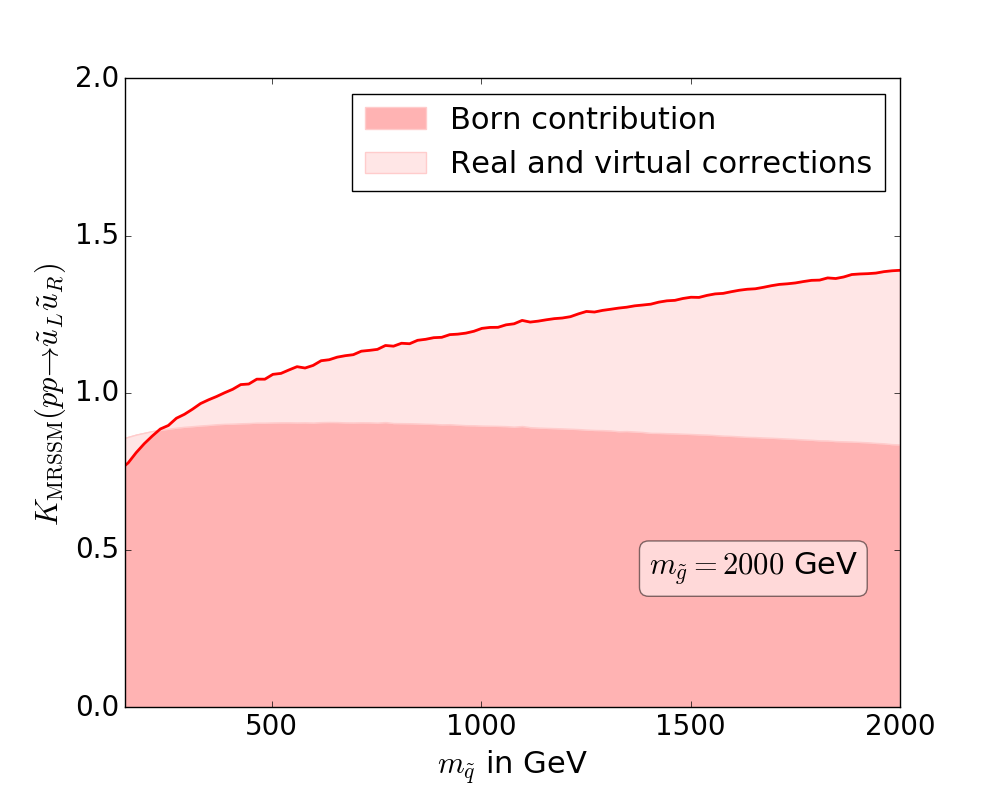
\includegraphics[scale=.5]{figures/MRSSM_uu_susu_Kfactors_msg=2000GeV.png}
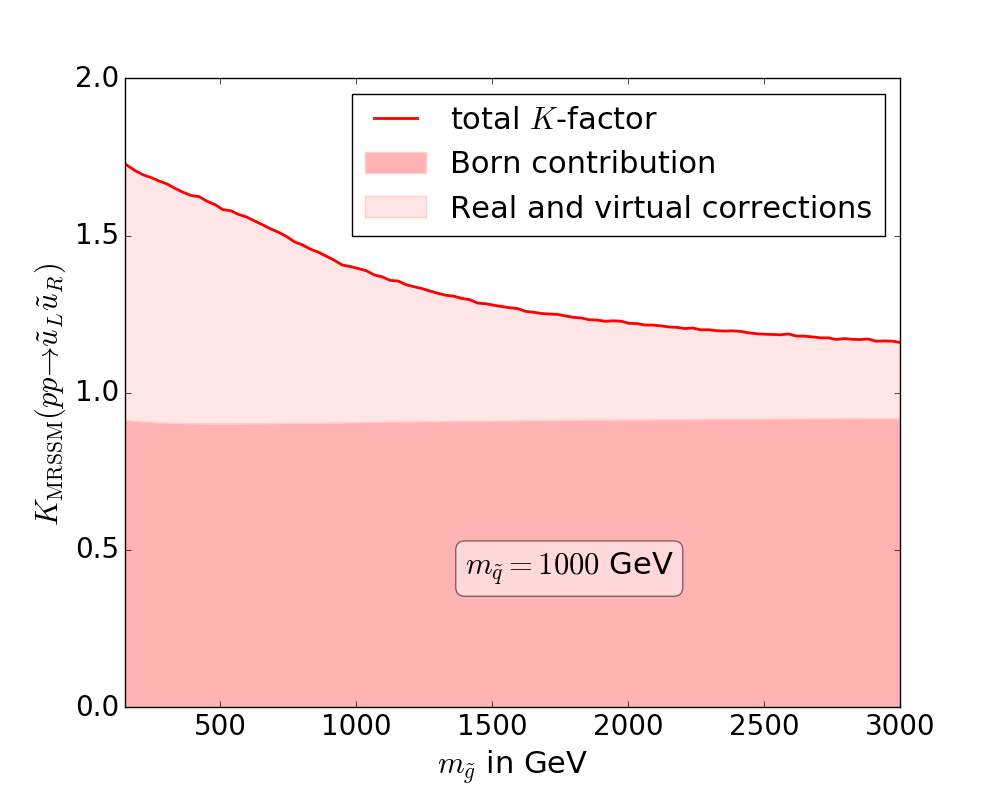
\includegraphics[scale=.5]{figures/MRSSM_uu_susu_Kfactors_msq=1000GeV.png}
\caption{Dependence of the $K$-factor for the process $uu \to \tilde{u}_L\tilde{u}_R$ in the MRSSM on the squark mass $m_{\tilde{q}}$ for fixed $m_{\tilde{g}} = \unit[2000]{GeV}$ (top) and on the gluino mass $m_{\tilde{g}}$ for fixed $m_{\tilde{q}} = \unit[1000]{GeV}$ (bottom).}\label{fig:1LXsection_fixed_m}
\end{center}
\end{figure}
Calculate uncertainties for multiple points(pdf, scale, integration)


\subsubsection{$K$-factors for Squark Production in the MSSM}
\begin{figure}[!htpb]
\begin{center}
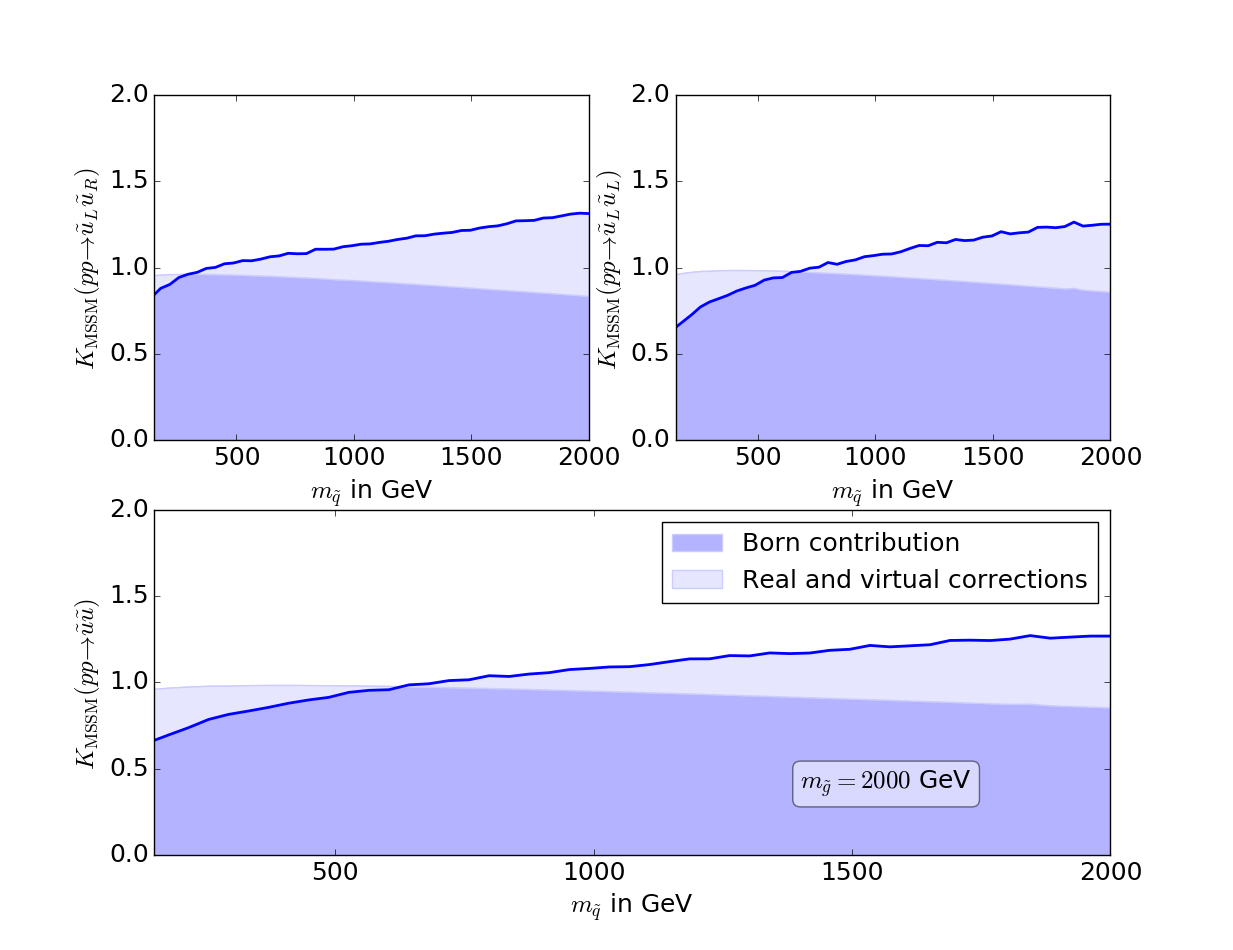
\includegraphics[scale=.5]{figures/MSSM_uu_susu_Kfactors_msg=2000GeV.png}
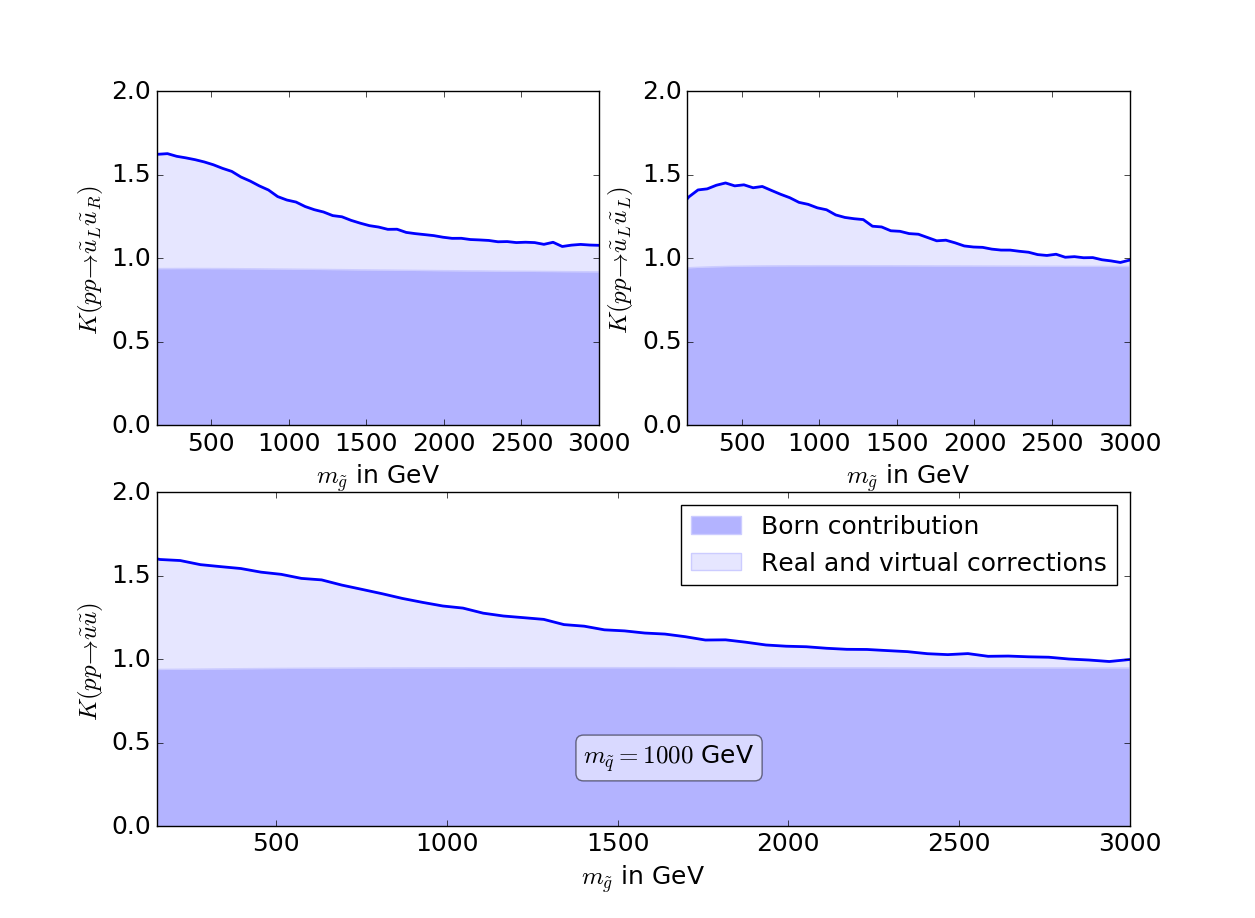
\includegraphics[scale=.5]{figures/MSSM_uu_susu_Kfactors_msq=1000GeV.png}
\caption{Dependence of the $K$-factor for the process $uu \to \tilde{u}\tilde{u}$, where $\tilde{u}\tilde{u} \in \left\{ \tilde{u}_L\tilde{u}_R, \tilde{u}_L\tilde{u}_L, \tilde{u}_R\tilde{u}_R \right\}$, in the MSSM on the squark mass $m_{\tilde{q}}$ for fixed $m_{\tilde{g}} = \unit[2000]{GeV}$ (top) and on the gluino mass $m_{\tilde{g}}$ for fixed $m_{\tilde{q}} = \unit[1000]{GeV}$ (bottom).}\label{fig:1LXsection_fixed_m}
\end{center}
\end{figure}
Calculate uncertainties for multiple points(pdf, scale, integration)
\texttt{MadGraph5\_aMC@NLO}\cite{Alwall:2014hca}
When generating the code for the process in question, e.g. two protons to $\tilde{u}_L + \tilde{u}_R$, with
\begin{lstlisting}[style=Mybash]
generate p p > ul ur [QCD] $$go
\end{lstlisting}
the $s$-channel gluinos were omitted as MadGraph does not deal with divergences coming from the gluino in the on-shell limit.




\subsection{The Cross Section in the Limit of Large Sgluon Masses}
The cross section for squark production does not exist in the limit of an infinitely large sgluon mass, instead it was found that it diverges logarithmically.\\
\begin{align}
\lim_{m_{\sigma}\to\infty} \sigma(qq \to \tilde{q}\tilde{q}) \sim \ln \frac{m_{\sigma}^2}{\mu^2}
\end{align}
This is actually expected as an effective field theory of the MRSSM where the sgluon is integrated out is no longer supersymmetric. This is because the sgluon is together with the octino part of a supermultiplet. Integrating out only the sgluon means that the octino misses its superpartner in the effective field theory. In this case the decoupling theorem \cite{Appelquist:1974tg} does no longer hold.\\
It is even possible to predict the  logarithmic scaling of $\sigma(qq \to \tilde{q}\tilde{q})$ quantitatively. The coefficient of the logarithm is proportional to the difference of the one-loop $\beta$ function coefficients of $g_s$ and $\hat{g}_s$ in the effective theory with the heavy particle integrated out, see eq. (4) in \cite{Cheng:1997sq}.
\begin{figure}[!htpb]
\begin{center}
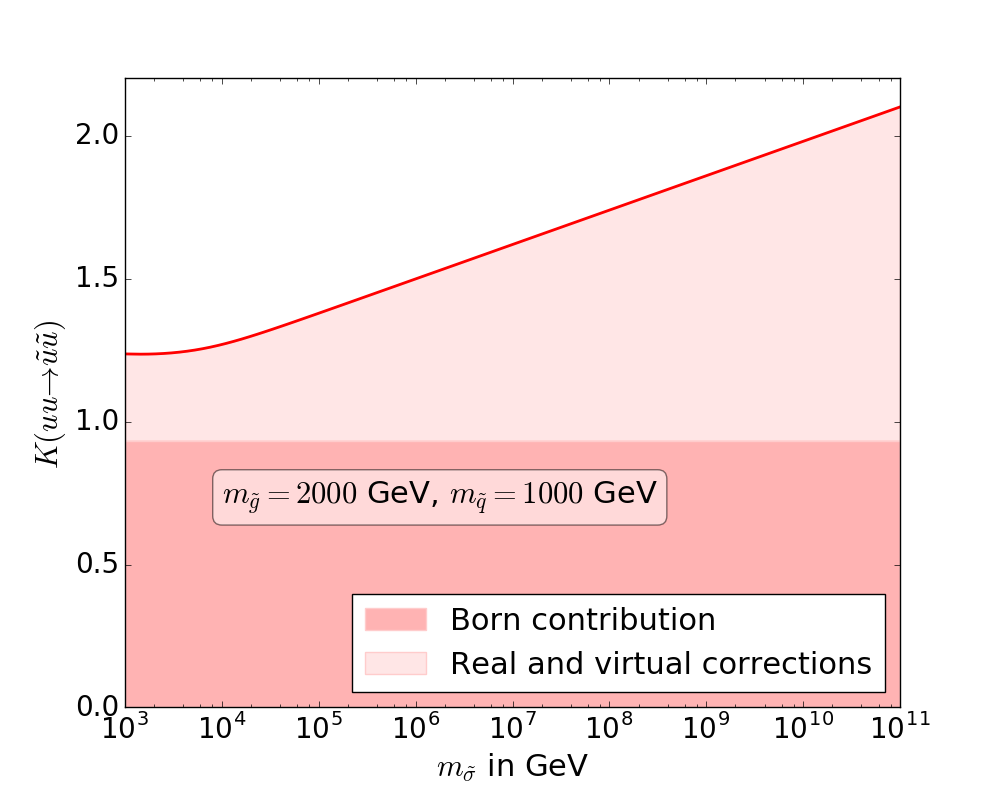
\includegraphics[scale=.5]{figures/MRSSM_uu_susu_Kfactors_msq=1000GeV_msg=2000GeV.png}
\caption{Dependence of the $K$-factor for the process $uu \to \tilde{u}\tilde{u}$ on the mass of the pseudoscalar sgluon. For $m_{\sigma} \approx \unit[10^5]{GeV}$ onwards want find a logarithmic scaling as predicted by \cite{Cheng:1997sq}.}
\end{center}
\end{figure}

